\section{Phase Space formalism}
\label{sec:ps}

\subsection{Stabilizer Theory}\label{sec:so}

Let $\{\ket{k}\}_{k \in \zd}$ be the standard computational basis for an arbitrary fault-tolerant scheme, defined over the finite field $\zd = \{ 0, 1, \dots,d-1 \}$, with $d$ an odd prime. 
Since the field has character $d$, addition and multiplication on the field are always considered modulo $d$.
The Hilbert space of any system associated with this scheme is $\hd \coloneqq \spanv{\ket{k}: k \in \zd}$.

The generalised Pauli matrices $X, Z$ can be defined by their respective roles as shift and phase operators,
\begin{align}
    X \ket{k} &= \ket{k + 1} \label{eq:xpauli}\\
	Z \ket{k} &= \omega^k \ket{k}, \label{eq:zpauli}
\end{align}
where $\omega \coloneqq e^{2\pi i/d}$ is the $d$-th root of unity. 

The Hilbert space $\hd$ is associated with a phase space $\pd \coloneqq \zd \times \zd$, where every point $\bmx \coloneqq (x_0, x_1)$ corresponds to a displacement operator, defined as
\begin{equation}\label{eq:ddef}
    D_{\bmx} \coloneqq \tau^{x_0 x_1} X^{x_0} Z^{x_1},\ \bmx  \in \pd.
\end{equation}
The phase factor $\tau \coloneqq -\omega^{1/2}$ ensures unitarity.
For a system with composite Hilbert space, $\hd = \hd[d_A] \otimes \hd[d_B]$, the displacement operators are defined as
\begin{equation}\label{eq:composited}
    D_{\bmx_A \oplus \bmx_B} \coloneqq D_{\bmx_A} \otimes D_{\bmx_B},
\end{equation}
where $\bmx_A \oplus \bmx_B \coloneqq (x_{A0}, x_{B0}, x_{A1}, x_{B1}) \in \pd[d_A] \times \pd[d_B]$.

The displacement operators, form a group under matrix multiplication modulo phases,
\begin{equation}\label{eq:gp}
    \gp \coloneqq \{ \tau^k D_{\bmz}: k \in \zd, \bmz \in \pd\}.
\end{equation}
The Clifford unitaries $\cd$ can then be defined as the normaliser of this group, \nick{Reformulate for copies of qudits: $\gp,\ \cd \rightarrow \gp^n,\ \cd^n$. $C-SUM$s live in $\cd^2$}
\begin{equation}
    \cd \coloneqq \{ U \in {\rm{SU}}(d): U\gp U^\dagger = \gp \}.
\end{equation}
The pure stabilizer states are then the orbit of the Clifford unitaries over a computational basis state,
\begin{equation}\label{eq:stab}
    \stab_{{\rm{pure}}} \coloneqq \{ U\ketbra{0}{0}U^\dagger: U \in \cd \}.
\end{equation}

The free states of the stabilizer theory are mixtures of pure stabilizers, 
\begin{equation}
    \stab = \conv\ \stab_{{\rm{pure}}}.
\end{equation}
The free operations of the stabilizer theory is the set of stabilizer operations $\so$ defined as any composition of:
\begin{enumerate}
    \item Preparation in computational basis;
    \item Random Clifford unitaries $\rcu$, i.e. operations $\E$ such that 
    \begin{equation}
        \E(\rho) = \sum_i p_i U_i \rho U_i^\dagger,\ U_i \in \cd;
\end{equation}
    \item Measurement in computational basis.
\end{enumerate}


\subsection{Wigner Distribution}\label{sec:wigner}

We can define the phase-point operators,
\begin{align}
	A_{\bmx} \coloneqq \frac{1}{d} \sum_{\bmz \in \pd} \omega^{\bmx \wedge \bmz} D_{\bmz},\ \bmx \in \pd. \label{eq:ax}
\end{align}
\nick{$\wedge$ has not be defined} They form an orthogonal Hermitian operator basis.
Therefore, any quantum state $\rho \in \cal{B}(\hd)$ can be expressed as a linear combination of the phase-point operators,
\begin{equation}
    \rho = \sum_{\bmz \in \pd} \W[\bmz]{\rho} A_{\bmz},
\end{equation}
where the coefficient vector $\W{\rho}$ is the Wigner distribution of state $\rho$,
\begin{equation}\label{eq:wstate}
    \W[\bmx]{\rho} \coloneqq \frac{1}{d}\tr[A_{\bmx} \rho].
\end{equation}
It is in fact a real, bounded, $d^2$-dimensional quasi-probability distribution over $\pd$ as shown in~\cref{app:wigner}. 

The Wigner distributions of different types of qutrit states are illustrated in~\cref{fig:wstate_examples}.
\begin{figure}%
    \centering
    \subfigure[][]{%
    \label{fig:maxmix}%
    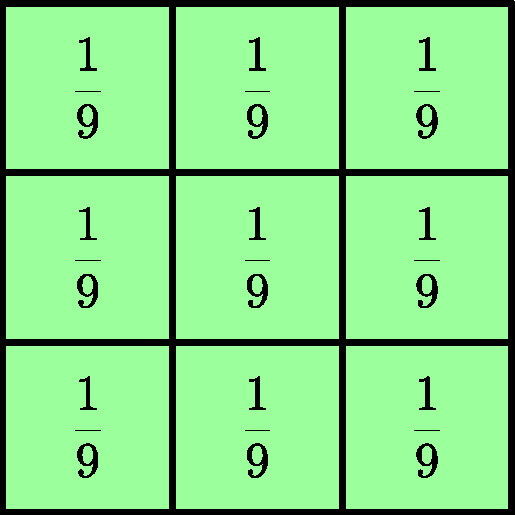
\includegraphics[height=2cm]{sections/magic/maxmixed.pdf}
    %\caption{Maximally mixed state $\frac{1}{3}\id$}%
    }\hspace{8pt}%
    \subfigure[][]{%
    \label{fig:zero}%
    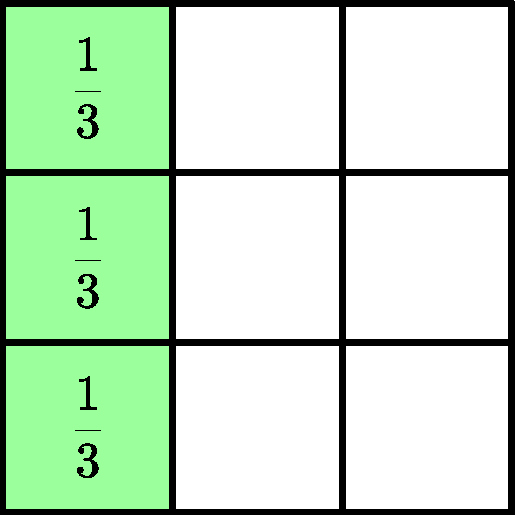
\includegraphics[height=2cm]{sections/magic/zerostate.pdf}
    %\caption{Zero state $\ketbra{0}{0}$}%
    }\\
    \subfigure[][]{%
    \label{fig:bound}%
    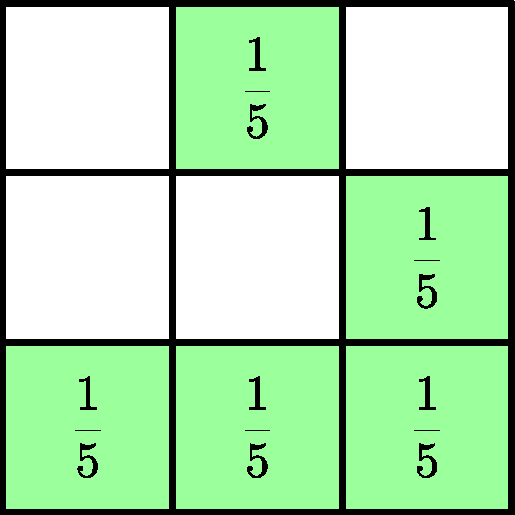
\includegraphics[height=2cm]{sections/magic/boundstate.pdf}
    %\caption{Bound state}%
    }\hspace{8pt}%
    \subfigure[][]{%
    \label{fig:strange}%
    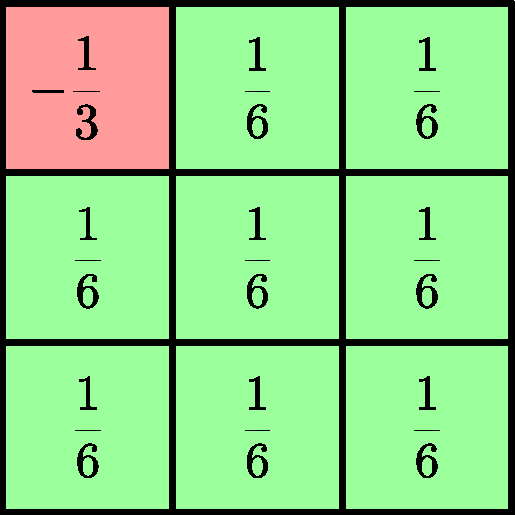
\includegraphics[height=2cm]{sections/magic/strangestate.pdf}
    %\caption{Strange state $\ketbra{S}{S}$}%
    }
    \caption{Wigner distributions for qutrit states of varying magic. 
    \subref{fig:maxmix} Maximally mixed state $\frac{1}{3}\id$; \subref{fig:zero} Stabilizer zero state $\ketbra{0}{0}$; \subref{fig:bound} A non-stabilizer Wigner-positive state; \subref{fig:strange} Magic strange state $\ket{{\rm{S}}} = \frac{1}{\sqrt{2}}(\ket{1} - \ket{2})$.
    \nick{Explain what a magic / bound magic state is in intro}
    }%
    \label{fig:wstate_examples}
\end{figure}

We can exploit the channel-state duality and use the normalised Choi-Jamio\l{}kowski state 
\begin{equation}\label{eq:cj}
    \frac{1}{d_A}\J_\E \coloneqq \frac{1}{d_A}(\id \otimes \E) \sum_{i,j} \ket{ii}\bra{jj}
\end{equation}
to extend the definition of the Wigner distribution to quantum $\cptp$ operations $\E: \cal{B}(\hd[d_A]) \mapsto \cal{B}(\hd[d_B])$, 
\begin{align}\label{eq:woperation}
    \W[\bmy|\bmx]{\E} 
    &\coloneqq d_A^2 \W[\bm{\bar x} \oplus \bmy]{\frac{1}{d_A}\J_\E} \\
    &= \frac{1}{d_B} \tr_B[A_{\bmy} \E(A_{\bmx})],
\end{align}
where $\bm{\bar x} \coloneqq (x_0, -x_1)$.

The specific form of~\cref{eq:woperation} is chosen so that Wigner distributions of operations act as transition matrices for Wigner distributions of states, $\W{\E(\rho)} = \W{\E}\W{\rho}$.
In particular, $\cptp$ operations that map between density operators of equal dimensions and have non-negative Wigner distributions correspond to stochastic matrices, as shown in~\cref{app:wigner}

The single-qudit Hadamard gate $H$ and phase gate $S$ generate the $d$-dimensional Clifford group $\cd$. \nick{CITE}
Their Wigner distributions are given by permutation matrices,
\begin{align}
    H &\coloneqq \frac{1}{\sqrt{d}}\sum_{j,k} \omega^{jk} \ketbra{j}{k}, \W[\bmy|\bmx]{H} = \delta_{y_0, -x_1}\delta_{y_1, x_0};\label{eq:H}\\
    S &\coloneqq \sum_k \tau^{k(k+1)} \ketbra{k}{k}, \W[\bmy|\bmx]{S} = \delta_{y_0, x_0}\delta_{y_1, x_0 + x_1 + 2^{-1}}.\label{eq:S}
\end{align}